\chapter{Results}
\label{chap:results}

\section{Augmentation Results}

\begin{table}[H]
\centering
\setlength{\tabcolsep}{4pt}
\renewcommand{\arraystretch}{1.25}
\scriptsize
\resizebox{\textwidth}{!}{%
\begin{tabular}{lccccccccc}
\toprule
\textbf{Model} & \textbf{BASE} & \textbf{GAUS} & \textbf{PINK} & \textbf{TEMP} & \textbf{SEGR} & \textbf{CHDO} & \textbf{MIXU} & \textbf{WGAN} & \textbf{LDIF} \\
\midrule

EEGNet 
& \makecell{0.6781 \\ 0.6330}
& \makecell{0.6795 \\ 0.6295}
& \makecell{0.6982 \\ 0.6499}
& \makecell{0.6858 \\ 0.6432}
& \makecell{\textbf{0.7072} \\ 0.6521}
& \makecell{0.6984 \\ 0.6459}
& \makecell{0.6941 \\ \textbf{0.6577}}
& \makecell{0.7001 \\ 0.6510}
& \makecell{0.6993 \\ 0.6475} \\
\midrule

EEGNeX
& \makecell{0.7164 \\ 0.6586}
& \makecell{0.7191 \\ 0.6585}
& \makecell{0.7354 \\ 0.6757}
& \makecell{0.7348 \\ 0.6778}
& \makecell{\textbf{0.7489} \\ \textbf{0.6874}}
& \makecell{0.7358 \\ 0.6601}
& \makecell{0.7361 \\ 0.6779}
& \makecell{0.7443 \\ 0.6806}
& \makecell{0.7435 \\ 0.6821} \\
\midrule

EEGInceptionERP
& \makecell{0.6568 \\ 0.6163}
& \makecell{0.6584 \\ 0.6245}
& \makecell{0.6720 \\ 0.6305}
& \makecell{0.6683 \\ 0.6303}
& \makecell{\textbf{0.6896} \\ \textbf{0.6420}}
& \makecell{0.6835 \\ 0.6319}
& \makecell{0.6780 \\ 0.6364}
& \makecell{0.6827 \\ 0.6359}
& \makecell{0.6809 \\ 0.6367} \\
\midrule

CNN-LSTM
& \makecell{0.7145 \\ 0.6510}
& \makecell{0.7257 \\ 0.6595}
& \makecell{0.7318 \\ 0.6645}
& \makecell{0.7300 \\ 0.6778}
& \makecell{\textbf{0.7405} \\ \textbf{0.6792}}
& \makecell{0.7358 \\ 0.6688}
& \makecell{0.7352 \\ 0.6733}
& \makecell{0.7386 \\ 0.6761}
& \makecell{0.7394 \\ 0.6763} \\
\midrule

EEGConformer
& \makecell{0.6512 \\ 0.6214}
& \makecell{0.6629 \\ 0.6136}
& \makecell{0.6784 \\ 0.6419}
& \makecell{0.6726 \\ 0.6455}
& \makecell{\textbf{0.6862} \\ 0.6490}
& \makecell{0.6748 \\ 0.6446}
& \makecell{0.6779 \\ 0.6308}
& \makecell{0.6835 \\ \textbf{0.6492}}
& \makecell{0.6806 \\ 0.6489} \\
\midrule

Average
& \makecell{0.6834 \\ 0.6360}
& \makecell{0.6891 \\ 0.6371}
& \makecell{0.7031 \\ 0.6525}
& \makecell{0.6983 \\ 0.6549}
& \makecell{\textbf{0.7144} \\ \textbf{0.6619}}
& \makecell{0.7056 \\ 0.6502}
& \makecell{0.7042 \\ 0.6552}
& \makecell{0.7098 \\ 0.6585}
& \makecell{0.7087 \\ 0.6583} \\
\midrule

$\Delta$ (\%)
& \makecell{0 \\ 0}
& \makecell{0.83 \\ 0.17}
& \makecell{2.88 \\ 2.59}
& \makecell{2.18 \\ 2.97}
& \makecell{\textbf{4.53} \\ \textbf{4.07}}
& \makecell{3.24 \\ 2.23}
& \makecell{3.04 \\ 3.01}
& \makecell{3.86 \\ 3.53}
& \makecell{3.70 \\ 3.50} \\
\bottomrule
\end{tabular}%
}
\caption{Combined comparison of model performance across augmentation settings. Each cell reports Macro F1 (top) and Macro PR AUC (bottom).}
\label{tab:combined_aug_results}
\end{table}

The results of the model-augmentation paired trainings are presented in Table~\ref{tab:combined_aug_results}. Each cell contains the Macro F1 and Macro PR AUC metrics for the corresponding pair, where the values represent the average of three different training runs.

All augmentation methods were able to consistently improve performance compared to the baseline setup. For each model, both the Macro F1 and Macro PR AUC scores increased with the use of augmentations with the only exception being Gaussian noise injection, which showed occasional drops in Macro PR AUC values. Pink noise resulted in noticeably higher performance gain than gaussian noise augmentation. This indicates that pink noise is more effective than Gaussian noise in improving model performance in the evaluated setup.

The highest overall performance was acchieved by SEGR, with largest relative improvement compared to the baseline, +4.53\% in Macro F1 and +4.07\% in Macro PR AUC. 

The two generative method also led to notable improvements. WGAN and the proposed LDIF achieved strong gains of +3.86\% and +3.70\% Macro F1 respectively. WGAN even resulted in highest Macro PR AUC score for EEGConformer, while MIXU achieved the top score for EEGNet. 

On model level, the global best performance was achieved by the EEGNeX, reaching a Macro F1 score of 0.7489. On the other hand, EEGNet shows the lowest overall performance across all models. 

Figure~\ref{fig:augmentation_delta} further highlights augmentation effects by comparing the relative performance gains of each method. The comparison between Macro F1 and Macro PR AUC gains shows that certain augmentations, such as MIXU, WGAN and LDIF, managed to achieve relatively balanced improvements across both metrics. Additionally, the relatively small variability of multiple runs indicates the consistency of the augmentation effects.

While all augmentation techniques are able to improve model performance in general, the magnitude of improvements differ across methods. Although SEGR achieves the highest scores, the proposed LDIF method remains competitive and consistent across all models.

\begin{figure}[H]
\centering
    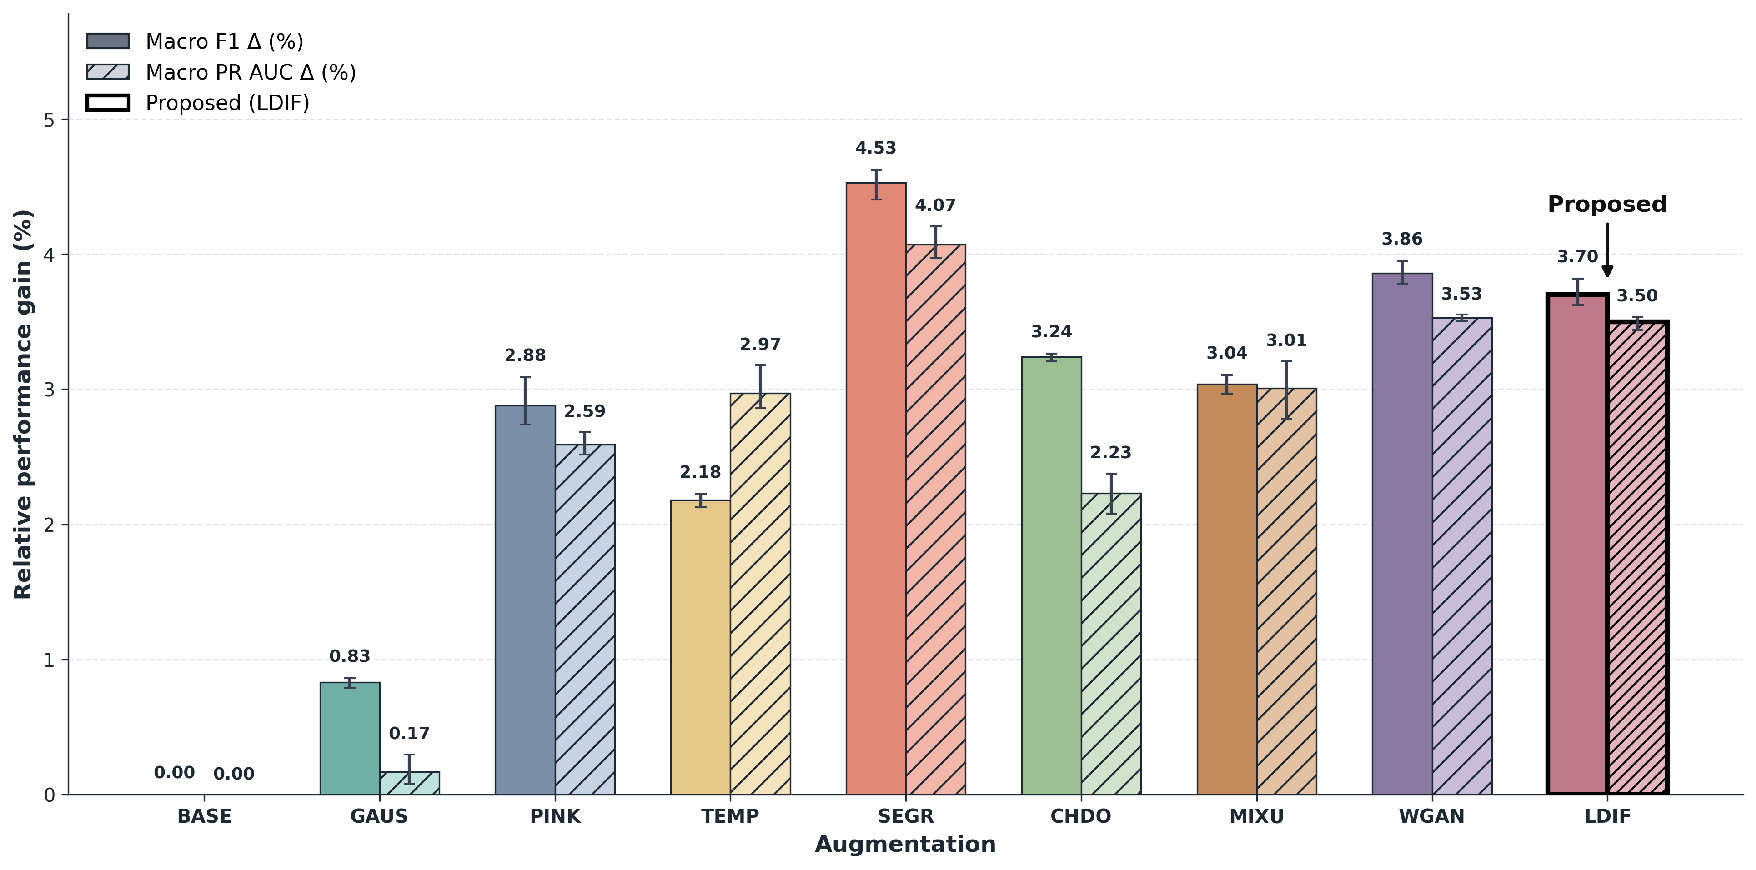
\includegraphics[width=1\textwidth]{images/augmentation_delta.pdf}
    \caption{Relative performance gains (\%) of augmentation methods compared to the baseline, measured in Macro F1 (solid) and Macro PR AUC (hatched). The proposed method (LDIF) is highlighted. Error bars indicate the min–max range across runs.}
    \label{fig:augmentation_delta}
\end{figure}

\section{Composition-Based Comparison}

\newcolumntype{C}[1]{>{\centering\arraybackslash}p{#1}}

\begin{table}[H]
\centering
\renewcommand{\arraystretch}{1.25}
\setlength{\tabcolsep}{3pt}

\resizebox{\textwidth}{!}{%
\begin{tabular}{@{}C{3cm}*{7}{C{2cm}}@{}}
\toprule
\textbf{Model} & 
\textbf{BASE} & 
\textbf{CAP} & 
\textbf{CPP} & 
\makecell{\textbf{CAP +}\\\textbf{WGAN}} & 
\makecell{\textbf{CPP +}\\\textbf{WGAN}} & 
\makecell{\textbf{CAP +}\\\textbf{LDIF}} & 
\makecell{\textbf{CPP +}\\\textbf{LDIF}} \\
\midrule

EEGNet
& \makecell{0.6781 \\ 0.6330}
& \makecell{0.7125 \\ 0.6609}
& \makecell{0.7089 \\ 0.6526}
& \makecell{0.7160 \\ 0.6658}
& \makecell{0.7143 \\ 0.6658}
& \makecell{\textbf{0.7175} \\ 0.6614}
& \makecell{0.7128 \\ 0.6598} \\
\midrule

EEGNeX
& \makecell{0.7164 \\ 0.6586}
& \makecell{0.7543 \\ 0.6846}
& \makecell{0.7498 \\ 0.6873}
& \makecell{\textbf{0.7555} \\ \textbf{0.6896}}
& \makecell{0.7486 \\ 0.6658}
& \makecell{0.7550 \\ 0.6860}
& \makecell{0.7510 \\ 0.6831} \\
\midrule

EEGInceptionERP
& \makecell{0.6568 \\ 0.6163}
& \makecell{0.6936 \\ 0.6487}
& \makecell{0.6907 \\ 0.6466}
& \makecell{\textbf{0.6977} \\ 0.6513}
& \makecell{0.6954 \\ 0.6507}
& \makecell{0.6924 \\ 0.6543}
& \makecell{0.6927 \\ \textbf{0.6612}} \\
\midrule

CNN-LSTM
& \makecell{0.7145 \\ 0.6510}
& \makecell{0.7491 \\ 0.6845}
& \makecell{0.7492 \\ 0.6824}
& \makecell{0.7481 \\ \textbf{0.6901}}
& \makecell{\textbf{0.7503} \\ 0.6880}
& \makecell{0.7481 \\ 0.6857}
& \makecell{0.7463 \\ 0.6828} \\
\midrule

EEGConformer
& \makecell{0.6512 \\ 0.6214}
& \makecell{0.6920 \\ 0.6548}
& \makecell{0.6919 \\ 0.6536}
& \makecell{0.6973 \\ \textbf{0.6589}}
& \makecell{\textbf{0.6954} \\ 0.6572}
& \makecell{0.6944 \\ 0.6561}
& \makecell{0.6920 \\ 0.6509} \\
\midrule

Average
& \makecell{0.6834 \\ 0.6360}
& \makecell{0.7203 \\ 0.6667}
& \makecell{0.7181 \\ 0.6645}
& \makecell{\textbf{0.7229} \\ \textbf{0.6711}}
& \makecell{0.7208 \\ 0.6655}
& \makecell{0.7214 \\ 0.6687}
& \makecell{0.7189 \\ 0.6675} \\
\midrule

$\Delta$ (\%)
& \makecell{0 \\ 0}
& \makecell{5.39 \\ 4.82}
& \makecell{5.07 \\ 4.48}
& \makecell{\textbf{5.77} \\ \textbf{5.51}}
& \makecell{5.47 \\ 4.63}
& \makecell{5.56 \\ 5.14}
& \makecell{5.19 \\ 4.95} \\
\bottomrule
\end{tabular}%
}
\caption{Combined comparison of model performance across combined augmentation settings. Each cell reports Macro F1 (top) and Macro PR AUC (bottom).}
\label{tab:combined_composition_results}
\end{table}

The results of the composition-based trainings are presented in Table~\ref{tab:combined_composition_results}. Similarly to the model-augmentation paired settings, all composition-based methods improved performance compared to the baseline across all models.

Both CAP and CPP further improved the scores compared to the previous experiment, corresponding to more than 5\% gains in Macro F1 and 4\% in Macro PR AUC score over the baseline. The introduction of generative augmentations improved upon these results, as the addition of both WGAN and LDIF increased the overall performance.

The combined method of CAP + WGAN resulted in the highest average performance gain, achieving +5.77\% in Macro F1 and +5.51\% in Macro PR AUC. While the addition of WGAN has the strongest effect on both CAP and CPP, LDIF also managed to produce top Macro F1 scores for EEGNet and top Macro PR AUC score for EEGInceptionERP. 

At model level, EEGNeX outperformed all other models, producing the global best Macro F1 score of 0.7555. This high score was achieved with the CAP + WGAN combined pipeline, while CAP + LDIF managed to produce a similar Macro F1 score of 0.7550.


\begin{figure}[H]
\centering
    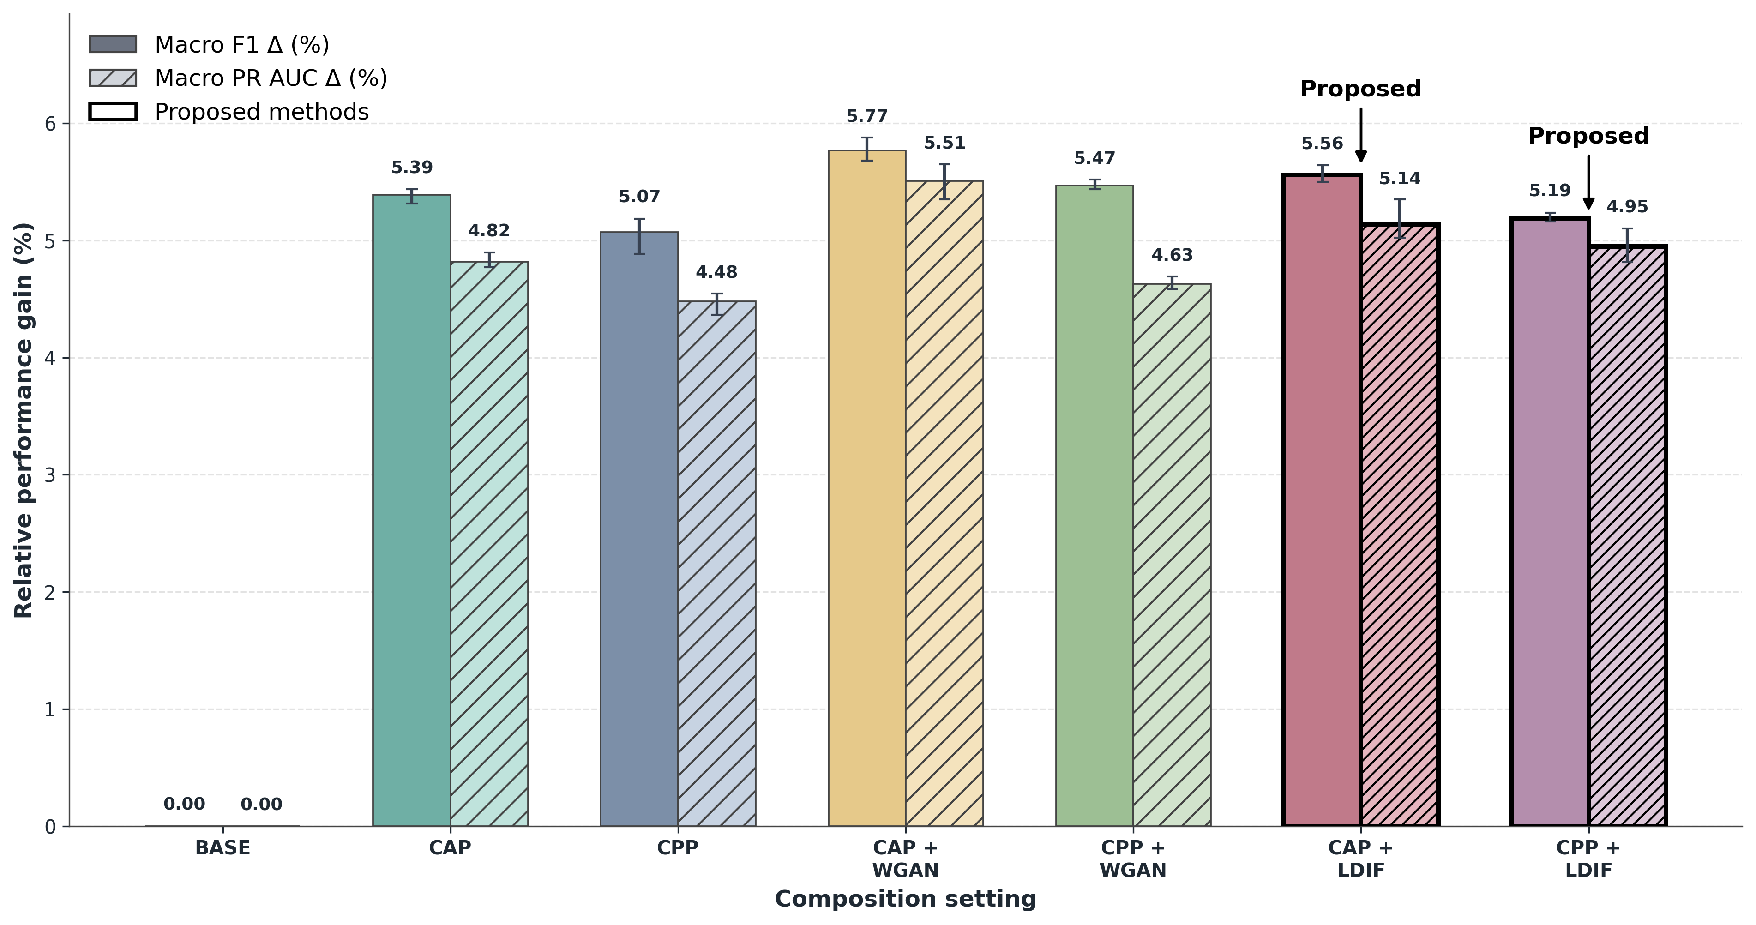
\includegraphics[width=1\textwidth]{images/augmentation_delta2.pdf}
    \caption{Relative performance gains (\%) of composition-based augmentation methods compared to the baseline, measured in Macro F1 (solid) and Macro PR AUC (hatched). The proposed methods are highlighted. Error bars indicate the min–max range across runs.}
    \label{fig:augmentation_delta2}
\end{figure}

Figure~\ref{fig:augmentation_delta} illustrates the effects of the combined methods by comparing the relative performance gains achieved using each method, and the narrow min-max range again shows the consistency of these gains.

While combinations including generative methods were able to further improve classification performance compared to CAP or CPP alone, the additional gains provided by these combinations were relatively modest.


\section{Additional Experiments}

The effectiveness of the proposed LDIF augmentation across different artifact classes is presented in Table~\ref{tab:combined_performance}. The results show improvements on all labels for both metrics. 

The highest improvement was achieved for the chew class with a +7.11\% gain in F1 score, while the models were also able to improve the classification of the elec label with gains of +3.42\% in F1 and +4.94\% in PR AUC. 

The proposed method could also achieve moderate improvement on the already well classified eyem label, reaching the highest F1 score of 0.8308 and the highest PR AUC of 0.7901, with gain of +2.59\% and +2.62\% respectively.

\begin{table}[H]
\centering

% ---------- F1 ----------
\begin{subtable}[t]{\textwidth}
\centering
\caption{F1 scores}
\renewcommand{\arraystretch}{1.2}
\setlength{\tabcolsep}{5pt}
\begin{tabular}{lccccc}
\hline
Setting & musc & eyem & elec & chew & Macro \\
\hline
BASE             & 0.7225 & 0.8098 & 0.7133 & 0.4880 & 0.6834 \\
LDIF         & 0.7438 & 0.8308 & 0.7377 & 0.5227 & 0.7087 \\
$\Delta$ (\%) & 2.94    & 2.59    & 3.42    & 7.11    & 3.70    \\
\hline
\end{tabular}
\end{subtable}

\vspace{0.4em}

% ---------- PR AUC ----------
\begin{subtable}[t]{\textwidth}
\centering
\caption{PR AUC scores}
\renewcommand{\arraystretch}{1.2}
\setlength{\tabcolsep}{5pt}
\begin{tabular}{lccccc}
\hline
Setting & musc & eyem & elec & chew & Macro \\
\hline
BASE             & 0.6397 & 0.7699 & 0.6310 & 0.5036 & 0.6360 \\
LDIF         & 0.6643 & 0.7901 & 0.6622 & 0.5166 & 0.6583 \\
$\Delta$ (\%) & 3.84    & 2.62    & 4.94    & 2.58    & 3.50    \\
\hline
\end{tabular}
\end{subtable}

\caption{Per-class comparison of baseline (BASE) and proposed (LDIF) performance, measured in (a) F1 and (b) PR AUC. The bottom row reports relative improvements (\%) of LDIF over the baseline.}
\label{tab:combined_performance}
\end{table}

Figure~\ref{fig:augmentation_delta3} highlights the relative performance gains across classes and shows the small variability across runs, which suggests stable and reproducible results. Together, these evaluation results provide an overview of the improvements achieved by the proposed generative augmentation technique, benefiting classification performance for both previously well classified and misclassified labels, improving overall performance across all artifacts. 
\newline

\begin{figure}[H]
\centering
    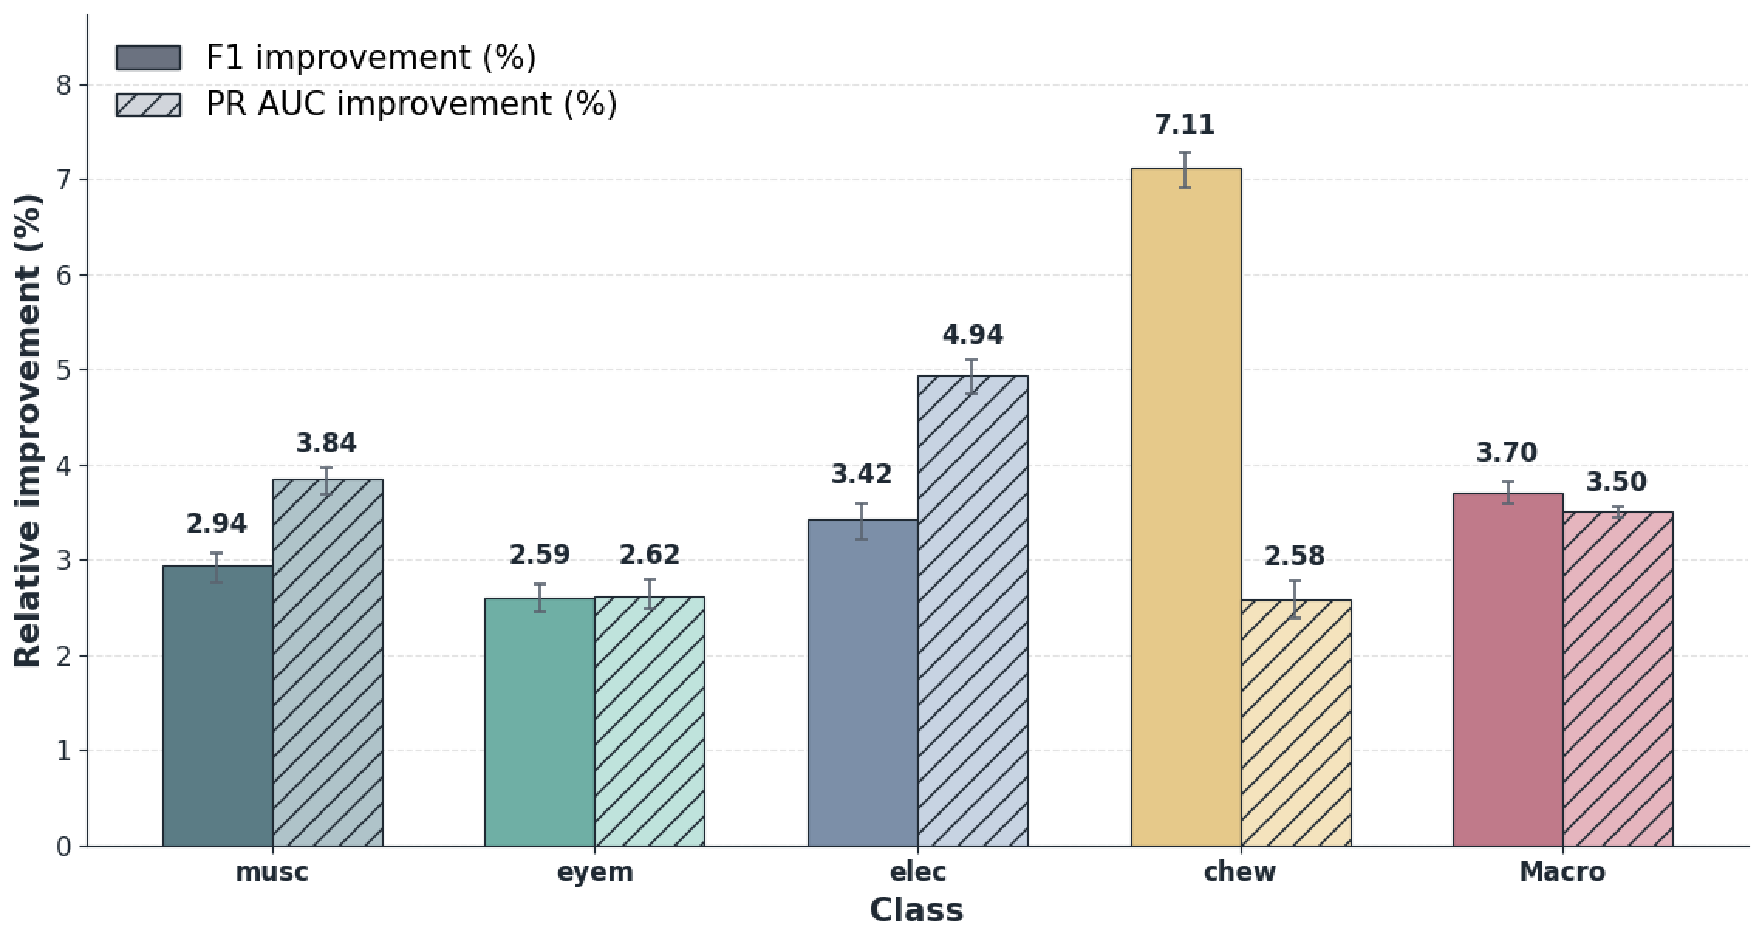
\includegraphics[width=0.9\textwidth]{images/augmentation_delta3.pdf}
    \caption{Relative improvement (\%) in classification performance across artifact classes, measured in F1 score (solid) and PR AUC (hatched). Error bars indicate the min–max range across runs.}
    \label{fig:augmentation_delta3}
\end{figure}
